\documentclass[a4paper,11pt]{jsarticle}

% 数式
\usepackage{amsmath,amsfonts}
\usepackage{amsthm}
\usepackage{bm}
\usepackage{mathtools}
\usepackage{amssymb}

% 表
\usepackage[utf8]{inputenc}
\usepackage{diagbox} % 斜線付きセルを作成するために必要
\usepackage{booktabs} % 表の罫線を美しくするために必要
\usepackage{hhline} % 水平罫線を制御するために必要

% 画像
\usepackage[dvipdfmx]{graphicx}
\usepackage{ascmac}
\usepackage{physics}
\usepackage{float} % 追加

% 図
\usepackage[dvipdfmx]{graphicx}
\usepackage{tikz} %図を描く
\usetikzlibrary{positioning, intersections, calc, arrows.meta,math} %tikzのlibrary

% ハイパーリンク
\usepackage[dvipdfm,
  colorlinks=false,
  bookmarks=true,
  bookmarksnumbered=false,
  pdfborder={0 0 0},
  bookmarkstype=toc]{hyperref}

% 式番号を章ごとにリセット
\numberwithin{equation}{section}

\begin{document}

\title{8章}
\author{大上由人}
\date{\today}
\maketitle

\setcounter{section}{7}
\section{くりこみ群}
\subsection{1次元Ising模型}
\subsubsection{粗視化}
1次元Ising模型において、一つおきのスピンについて和をとるという粗視化を行う。
いま、$K = \beta J$, $H = \beta h$とおくと、分配関数は、
\begin{align}
    Z = \sum_{S_1, S_2, \cdots, S_N} \exp \qty(K \sum_{i=1}^{N-1} S_i S_{i+1} + H \sum_{i=1}^{N} S_i)
\end{align}
であった。ただし、スピン数$N$は偶数であるとし、周期的境界条件$S_{N+1} = S_1$を課す。ここで、偶数番目のスピンについて和をとることを考える。例えば、$S_2$について和をとってみると、
\begin{align}
    \sum_{S_2} \exp \qty(K S_1 S_2 + K S_2 S_3 + H S_2) = \exp(K S_1 + H + K S_3) + \exp(-K S_1 - H - K S_3)
\end{align}
となる。ここで、この右辺は$S_1, S_3$を含む関数になっているが、$S_i^2 = 1$であることを踏まえると、うまく定数を合わせれば、
\begin{align}
    \exp(A' + \frac{\delta}{2} S_1 + K'S_1 S_3 + \frac{\delta H}{2} S_3) 
\end{align}
と書ける。ただし、$A', \delta, K', \delta H$は適当な定数である。これを用いて分配関数を書きなおすと、
\begin{align}
    Z(K,H,N) &= \sum_{S_1, S_3, \cdots, S_N}  \prod_{i=1}^{N/2} \exp(A' + \frac{\delta H}{2} S_{2i-1} + K' S_{2i-1} S_{2i+1} + \frac{\delta H}{2} S_{2i+1}) \exp(HS_{2i-1}) \\
    &= \exp(NA'/2) Z(K', H', N/2)
\end{align}
となる。ただし、$H' = H + \delta H$である。\footnote{周期的境界条件に気を付けて計算する。}よって、偶数番目だけの和をとることによって、奇数番目だけから構成される分配関数と、他の積の形になることがわかる。これを繰り返すことによって、スピンの数を半分にしていくことができる。
新たに得た奇数番目の分配関数に出てくる$K',H'$を具体的に求める。今、転送行列を比較することによって、\footnote{
    ここで、転送行列とは、
    \begin{align}
        \hat{T} = 
        \begin{pmatrix}
            e^{K+H} & e^{-K} \\
            e^{-K} & e^{K-H}
        \end{pmatrix}
    \end{align}
    である。
    \begin{align}
        \ket{S_i} &= \mqty(1\\0) \quad \text{if} \quad S_i = 1\\
        \ket{S_i} &= \mqty(0\\1) \quad \text{if} \quad S_i = -1
    \end{align}
    とすると、
    1次元Ising模型の分配関数を、
    \begin{align}
        Z &= \sum_{S_i = \pm 1} \cdots \sum_{S_N = \pm 1} \prod_{i=1}^{N} \bra{S_i}T\ket{S_{i+1}}\\
        &= \sum_{S_1 = \pm 1} \cdots \sum_{S_N = \pm 1} \bra{S_1}T\ket{S_2}\bra{S_2}T\ket{S_3}\cdots\bra{S_N}T\ket{S_1}\\
        &= \Tr(T^N)
    \end{align}
    と書くことができる。
}
\begin{align}
    \hat{T}^2 &= 
\left( 
\begin{pmatrix}
e^{K+H} & e^{-K} \\
e^{-K} & e^{K-H}
\end{pmatrix}
\right)^2 
\\
&=
\begin{pmatrix}
e^{2K+2H} + e^{-2K} & e^{H} + e^{-H} \\
e^{2K-2H} + e^{-2K} & e^{H} + e^{-H}
\end{pmatrix}
\\
&=
e^{A'}
\begin{pmatrix}
e^{K'+H'} & e^{-K'} \\
e^{-K'} & e^{K'-H'}
\end{pmatrix}
\end{align}
となる。よって、
\begin{align}
    e^{4K'} &= \frac{\cosh(2K+H) \cosh(2K-H)}{\cosh^2 H}\\
    e^{2H'} &= e^{2H} \frac{\cosh(2K+H)}{\cosh(2K-H)}\\
    e^{4A'} &= 16 \cosh(2K+H) \cosh(2K-H) \cosh^2 H
\end{align}
となる。ここで、粗視化の操作により、$K,H$がどのように変化していくかをみていく。特に代表的な場合として、以下の4つの場合を考える。\\
\textbf{$H=0$の場合}\\
このとき、
\begin{align}
    e^{2K'} &= \cosh(2K)\\
    H' &= 0
\end{align}
となる。このとき、$K$を変化させると、$K'$は以下のように変化する。
\begin{figure}[H]
    \begin{center}
    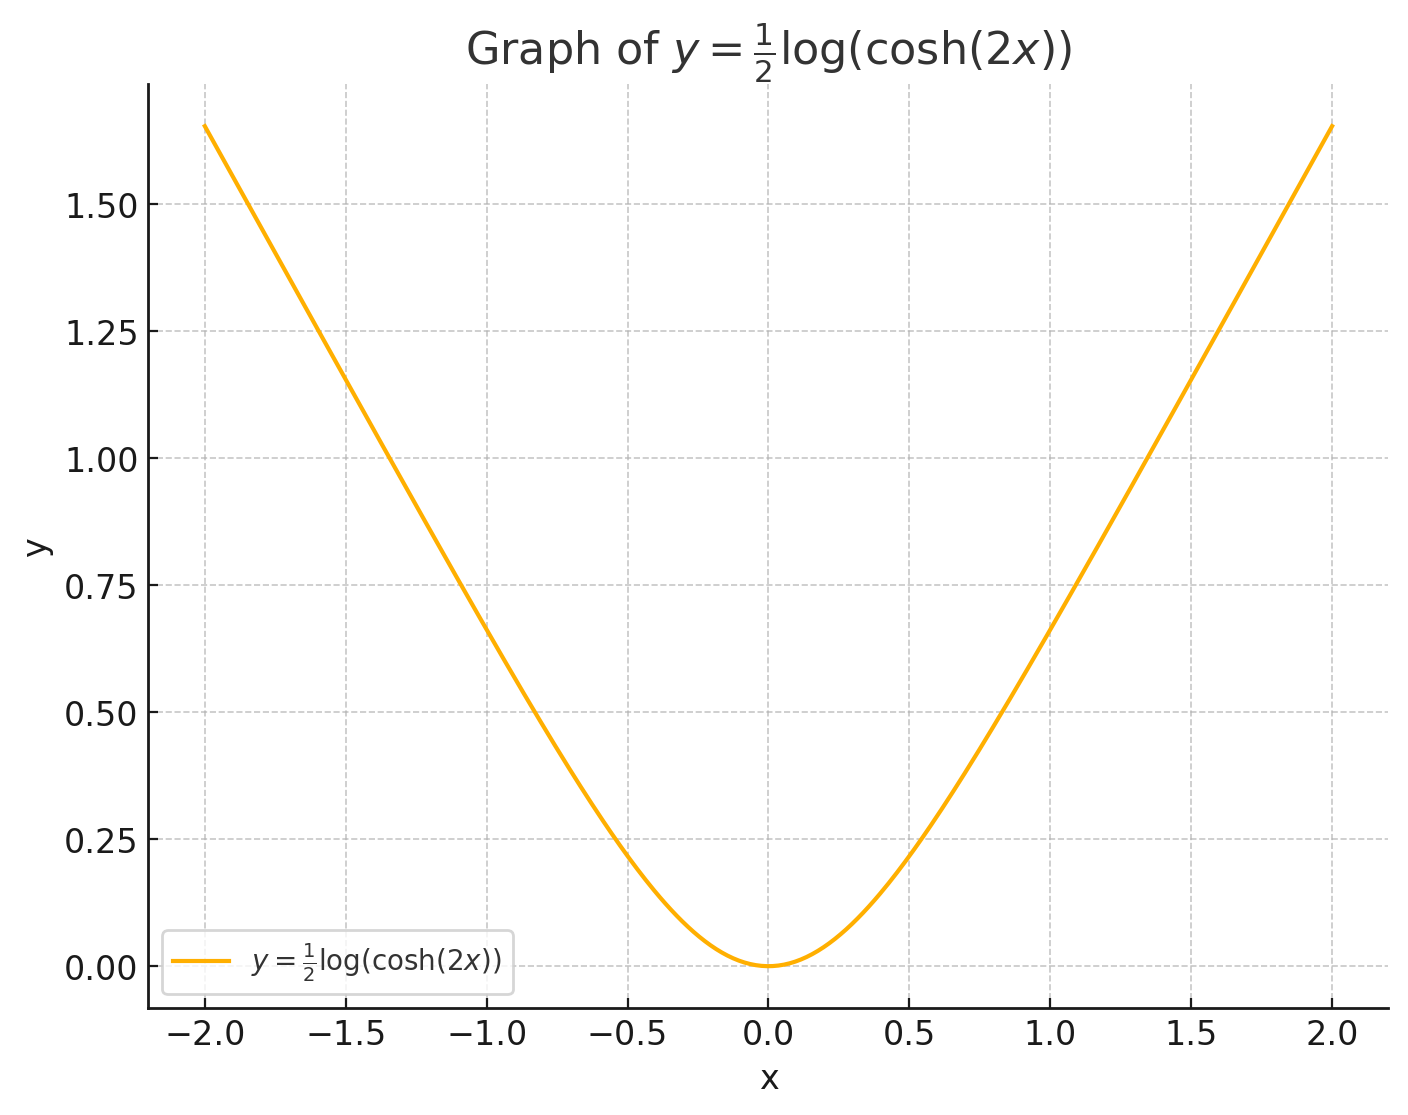
\includegraphics[width=100mm]{H0.png}
    \end{center}
    \caption{H=0の場合}
    \label{fig:one}
\end{figure}
したがって、$K>0$ならば、粗視化を繰り返すことで、この値は減少することがわかる。\footnote{$y=x$と比較する。}また、$K=0$においては$K'$も0になる。\\

\textbf{$K=0$の場合}\\
このとき、
\begin{align}
    K' &= 0\\
    H' &= H
\end{align}
となる。

\textbf{$K \to \infty$の場合}\\
このとき、
\begin{align}
    \label{eq:K}
    e^{2K'} &\sim \frac{e^{4K}}{4\cosh^2 H}\\
    H' &\sim 2H 
\end{align}
となる。このとき、$K'$は無限大のままで、$H'$は2倍になる。ただし、$H$が0のときは、$H'$も0になる。\\

\textbf{$H \to \infty$の場合}\\ 
このとき、
\begin{align}
    e^{4K'} &\to 1\\
    H' &\sim H
\end{align}
となる。このとき、$K'$は0に近づくが、磁場は変化しない。\\

これらの振る舞いをまとめると、以下の相図にまとめられる。
\begin{figure}[H]
    \begin{center}
    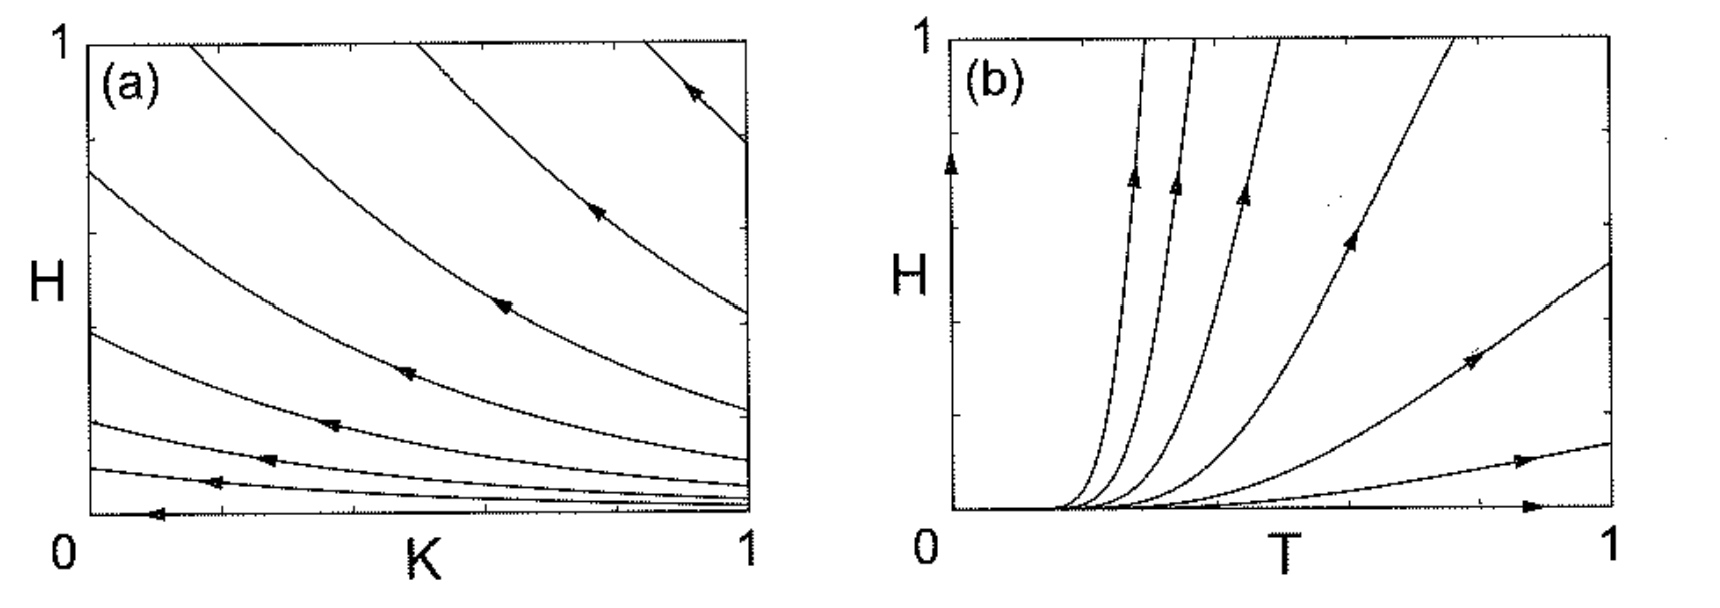
\includegraphics[width=120mm]{s.png}
    \end{center}
    \caption{相図}
    \label{fig:two}
\end{figure}
ただし、$T = \frac{1}{K}$である。それぞれの曲線は、
\begin{align}
    e^{2K}\sinh{H} = \text{const.} \label{eq:one}\\
\end{align}
となる。(導出は後で述べる。)\\
流れを見てみると、全体的に$K$は減少し、$H$は増加することがわかる。\\
$K = \beta J$が小さくなるということは、$J$を基準にした温度が高くなっていることを表している。$J$はハミルトニアンの中でもスピンをそろえようとする項の係数であったから、これは、粗視化により、
系が無秩序な状態になっていることを表している。一方で、$H = \beta h$が大きくなるということは、粗視化により、磁場が大きくなっていることを表している。これらからわかるように、粗視化は、系の特徴を増幅させる効果がある。\\
また、$K = \infty, H = 0$の点は、粗視化を行っても変化しない点である。粗視化の立場から、この点は特別な状態にあると考えることができる。\\

((\ref{eq:one})の導出)\\
\begin{align}
    e^{4k'} \sinh^2 H' &= \frac{\cosh(2K+H) \cosh(2K-H)}{\cosh^2 H} \sinh^2 H'
\end{align}
である。ここで、
\begin{align}
    \sinh^2 H' &= \frac{1}{4} \qty(e^{2H'} -2 + e^{-2H'})\\
    &= \frac{1}{4} \qty(e^{2H}\frac{\cosh(2K+H)}{\cosh(2K-H)} -2 + e^{-2H}\frac{\cosh(2K-H)}{\cosh(2K+H)})
\end{align}
であることを用いると、
\begin{align}
    e^{4K'} \sinh^2 H' &= \frac{1}{4} \qty(\frac{\cosh^2(2K+H)}{\cosh^2 H}e^{2H} -2\frac{\cosh(2K+H)\cosh(2K-H)}{\cosh^2 H} + \frac{\cosh^2(2K-H)}{\cosh^2 H}e^{-2H})\\
    &= \frac{1}{4\cos^2 H} \qty(\cosh^2(2K+H)e^{H} -\cosh(2K-H)e^{-H})^2\\
    &= \frac{e^{4K}\sinh^2 H}{4} \qty(\frac{\cosh(2K+H)e^{H} - \cosh(2K-H)e^{-H}}{\sinh H \cosh H e^{2k}})^2
\end{align}
となる。また、
\begin{align}
    \frac{\cosh(2K+H)e^{H} - \cosh(2K-H)e^{-H}}{\sinh H \cosh H e^{2k}} &= e^{H-2K}\qty(\frac{\cos(2K)}{\sinh H} + {\sinh(2K)}\cosh H)\\
    &\quad -e^{-H-2K}\qty(\frac{\cos(2K)}{\sinh H} - {\sinh(2K)}\cosh H)\\
    &= \frac{\cosh(2K)}{\sinh H} e^{-2K} 2\sinh H \\
    &\quad+ \sinh(2K) \cosh H e^{-2K} 2\cosh H\\
    &= 2e^{-2K} (\cosh(2K) + \sinh(2K) )\\
    &= 2
\end{align}
となる。よって、
\begin{align}
    e^{4K'} \sinh^2 H' = e^{4K} \sinh^2 H
\end{align}
となる。\qed\\

\subsubsection{スケーリング}
前節では、臨界点付近のみについて観察していた。せっかくなので、ここでも、臨界点である$K = \infty $、$H = 0$における振る舞いを見てみる。
(\ref{eq:K})をさらに近似することで、
\begin{align}
    e^{4K'} &\sim \frac{1}{4}e^{4K}\\
    H' &\sim 2H
\end{align}
となる。いま、隣り合う格子をひとまとめにしていることを思い出すと、系のスケール変化は$x \to \frac{x}{2}$となるので、$b = 2$となる。このときの、磁場と温度のスケーリング次元を考える。\\
磁場については、上の式と$H' = b^{x_H}H$を比較することで、$x_H = 1$となる。\\
温度については少し工夫が必要である。6章の結果を用いると、相関長は、$\beta \to \infty$で、
\begin{align}
    \xi \sim e^{2K}
\end{align}
のように発散してしまう。このようなことが起きないように、適切に基本変数を選ぶ必要がある。
ここでは、基本変数として、$e^{-4K}$を用いることにすると、
\begin{align}
    e^{-4K'} \sim 4e^{-4K}
\end{align}
であるから、$x_t = 2$となる。このとき、臨界指数は、
\begin{align}
    \alpha &= 2- \frac{d}{x_t} = 2- \frac{1}{2} = \frac{3}{2}\\
    \beta &= \frac{d - x_H}{x_t} = \frac{1-1}{2} = 0\\
    \gamma &= \frac{2x_H - d}{x_t} = \frac{2-1}{2} = \frac{1}{2}\\
    \delta &= \frac{x_H}{d-x_H}  = \infty\\
    \nu &= \frac{1}{x_t} = \frac{1}{2}\\
    \eta &= d + 2 - 2x_H = 1
\end{align}
となる。\footnote{1次元なので$d=1$である。}
これらの臨界指数は、1次元Ising模型において、厳密に求まる結果と一致する。

また、1次元Ising模型は自由エネルギーが厳密に求まる。6章の結果を借用すると、
\begin{align}
    -\beta f = \ln(\cosh H + \sqrt{\sinh^2 H + t}) + K
\end{align}
となる。$t\ll 1, H\ll 1$の極限で、
\begin{align}
    -\beta f \sim t^{1/2}\qty(1 + \qty(\frac{H}{t^{1/2}})^2)^{1/2}
\end{align}
となる。教科書(7.68)式と見比べて、スケーリング関数が
\begin{align}
    \mathcal{F}(z) = \sqrt{1+z^2}
\end{align}
となることがわかる。


\subsection{くりこみ群の一般論}
粗視化の手続きをくりこみ群変換として表現することを考える。この手続きは、\textbf{自由度の部分的消去}と\textbf{空間のスケール変換}の二つの操作からなる。\\

\textbf{自由度の部分的消去}\\
考えている形の長さの最小スケールを$a$としたとき、$ba$以下のスケールの自由度を消去する。(たとえば、一次元Ising模型において、自由度$ba = 2a$以下のスケールの自由度を消去したのであった。)\\
自由度の消去の仕方は複数通りある。例えば、先ほどの1次元Ising模型のように、部分的にスピンの和をとる方法をデシメーションという。デシメーションを行うと、分配関数は以下のように書ける:
\begin{align}
    Z = \Tr_S \exp(\mathcal{H}(K,S)) &= \Tr_{S\circ} \Tr_{S\bullet} \exp(\mathcal{H}(K,S\circ, S\bullet))\\
    &= \Tr_{S\circ} \exp(\mathcal{H}'(K',S\circ))
\end{align}
ただし、$S_\bullet$は消去した自由度であり、$S\circ$は残した自由度である。一般には、$\mathcal{H}'$は二体相互作用に限らず、多体相互作用を含むこともある。\\
他にも、自由度の消去の仕方として、ブロックスピン変換と呼ばれるものがある。これは、二次元正方格子状のスピンについて、四つのスピン変数を一つの有効スピンに置き換えるというものである。\\
\begin{figure}[H]
    \begin{center}
    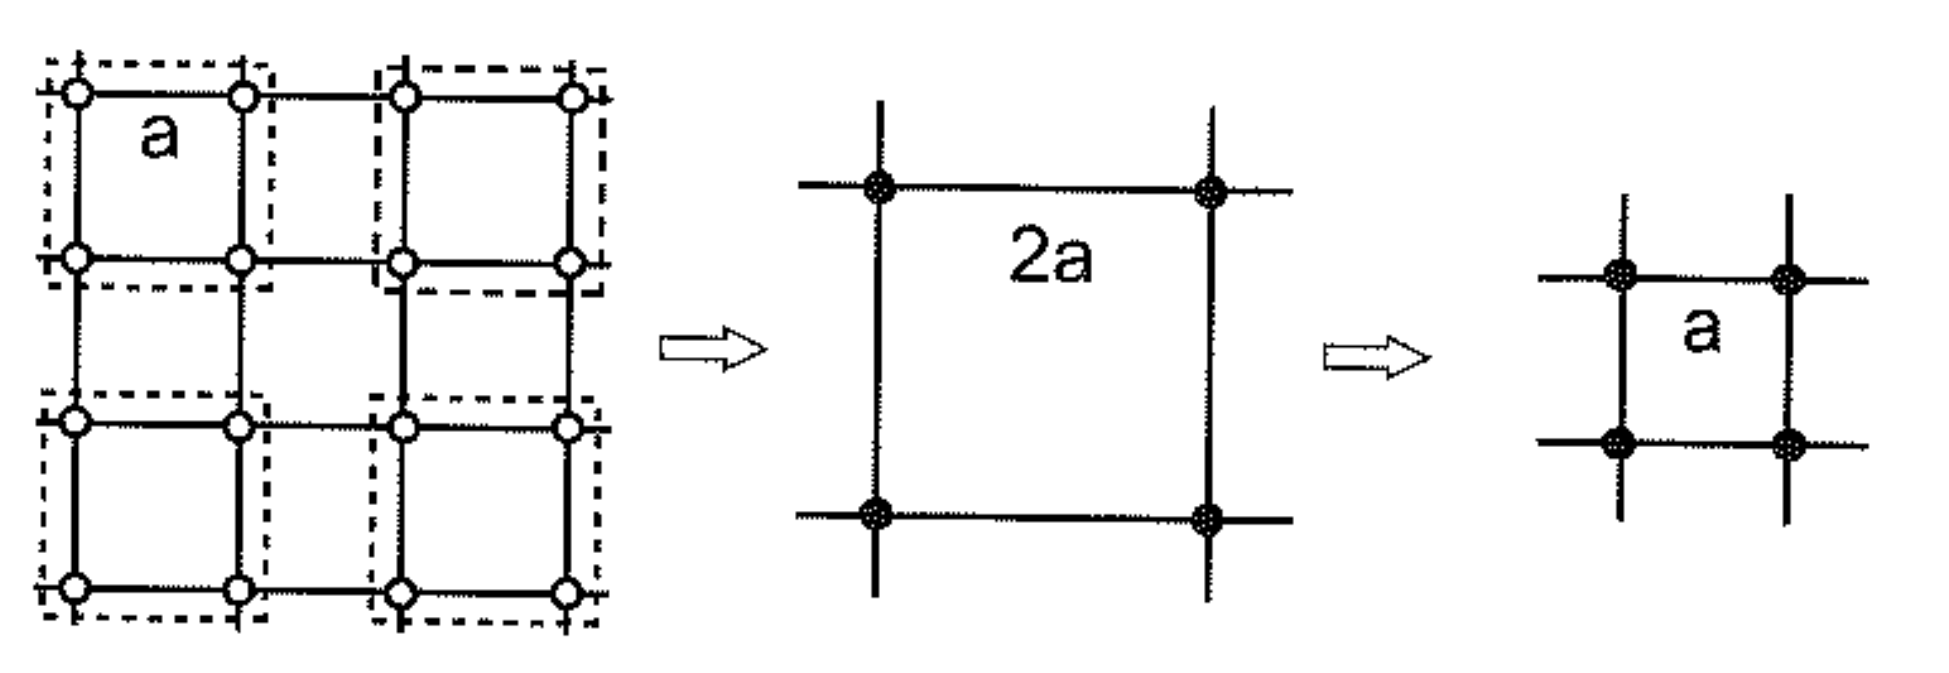
\includegraphics[width=100mm]{spin.png}
    \end{center}
    \caption{ブロックスピン変換}
    \label{fig:spin}
\end{figure}
このとき、スケール変換パラメータは$b=2$となる。一般に、ブロックスピン変換において、変数変換は$P(S',S)$を用いて表される。これは、ある$S$が与えられたとき、ある$S'$に対して1となり、それ以外の$S'$に対して0となる関数である。(要するに、所属先と対応していたら1、そうでなければ0となる関数)
よって、$\Tr_{S'} P(S',S) = 1$となる。このとき、分配関数は、
\begin{align}
    Z = \Tr_S \exp(\mathcal{H}(K,S)) &= \Tr_{S'} \Tr_S P(S',S) \exp(\mathcal{H}(K,S))\\
    &= \Tr_{S'} \exp(\mathcal{H}'(K',S'))
\end{align}
と書ける。ただし、
\begin{align}
    \exp(\mathcal{H}'(K',S')) := \Tr_S P(S',S) \exp(\mathcal{H}(K,S))
\end{align}
とした。\\
また、連続場の系についても、同様の操作ができる。連続場$\phi(\vb{r})$について、これをFourier変換し、波数空間でくりこみ群変換を行う。いま、これをFourier変換すると、
\begin{align}
    \phi(\vb{r}) = \int_{|\vb{k}| < \Lambda} \frac{d^d \vb{k}}{(2\pi)^d} \tilde{\phi}(\vb{k}) e^{i\vb{k}\cdot \vb{r}}
\end{align}
となる。このとき、$\Lambda$は最大波数である。このとき、$\Lambda/b < |\vb{k}| < \Lambda$の波数を持つ自由度を消去することを考える。これは、短いスケールのゆらぎを消去することに相当する。このようなくりこみ群を、運動量空間くりこみ群という。\\

\textbf{空間のスケール変換}\\
自由度の部分的消去を行った後、元の系のスケールに戻す必要がある。このとき、空間座標を$\vb{r} \to \frac{\vb{r}}{b}$とし、波数を$\vb{k} \to b\vb{k}$とする。
ブロックスピン変換においては図(\ref{fig:spin})のように行う。\\
運動量空間くりこみ群変換においては、$\vb{k} \to b\vb{k}$とすることにより、波数の上限が$\Lambda/b$から$\Lambda$になる。これにより、系のスケールがもとに戻る。\\

以上の二つの変換をもって、くりこみ群変換と呼ぶ。このときの結合定数の変化を、
\begin{align}
    K' = R_b(K)
\end{align}
と書く。このとき、この変換は以下の性質を満たす:
\begin{align}
    R_1(K) = K\\
    R_{b_1} \circ R_{b_2} = R_{b_1b_2}
\end{align}
したがって、この変換は半群をなす。

くりこみ群変換による自由エネルギーの変化は、
\begin{align}
    f(K) &= \frac{1}{V} \log Z_N(K)\\
    &=b^{-d} \frac{1}{Vb^{-d}} \log Z_{Nb^{-d}}(K)\\
    &= b^{-d} f(K')
\end{align}
となる。ただし、分配関数がくりこみ群変換に対して不変であることを用いた。これは、スケーリング理論における関係を一般化したものになっている。\\
スケーリング理論と異なる点は、臨界点に近い領域に限らず、任意の結合定数に対してくりこみ群変換を行えること、そして、変換が元の系にはなかった形の相互作用を作り出し得ることである。\\
くりこみ群変換の本質的な部分は、短いスケールの揺らぎを、結合定数の変化に押し付けることである。これにより、平均場理論で扱うことのできなかったゆらぎの効果を計算することができる。\\

\subsubsection{くりこみ群の流れと固定点}
くりこみ群変換による結合定数の変化を相図で追うことができる。

くりこみ群において、変換によってその値を変えない点(固定点)は重要である。
\begin{itembox}[l]{\textbf{Def.固定点}}
    くりこみ群変換によってその値を変えない点、すなわち、
    \begin{align}
        K^* = R(K^*)
    \end{align}
    を満たす点のことを固定点という。
\end{itembox}
くりこみ群変換を繰り返すことにより、相図上の任意の点はどこかの固定点に行きつき、そこの留まると考えられる。\footnote{閉軌道に収束する場合についてはこの本では考えない。}
このとき、その点が流れ込む固定点によってあらわされる系の性質が、その点の系の性質を表すと考える。
また、流れ込みのないような固定点を考えることもできる。そのような点では、他のどのような相図上の点もその点にたどり着くことができないのだから、相関長は無限大となる。ところで、Ising模型の例でも取り扱ったように、例えば臨界点においては磁化率は発散し、それは相関長が発散することに対応するのであった。
したがって、このような固定点は特に我々が関心のあるような点であることがわかる。流れ込みのない固定点のことを臨界固定点という。\\
これを拡張した概念として、臨界面や、さらに一般化した臨界多様体というものも考えることができる。\\
くりこみの流れを表した相図の例を以下に示す。
\begin{figure}[H]
    \begin{center}
    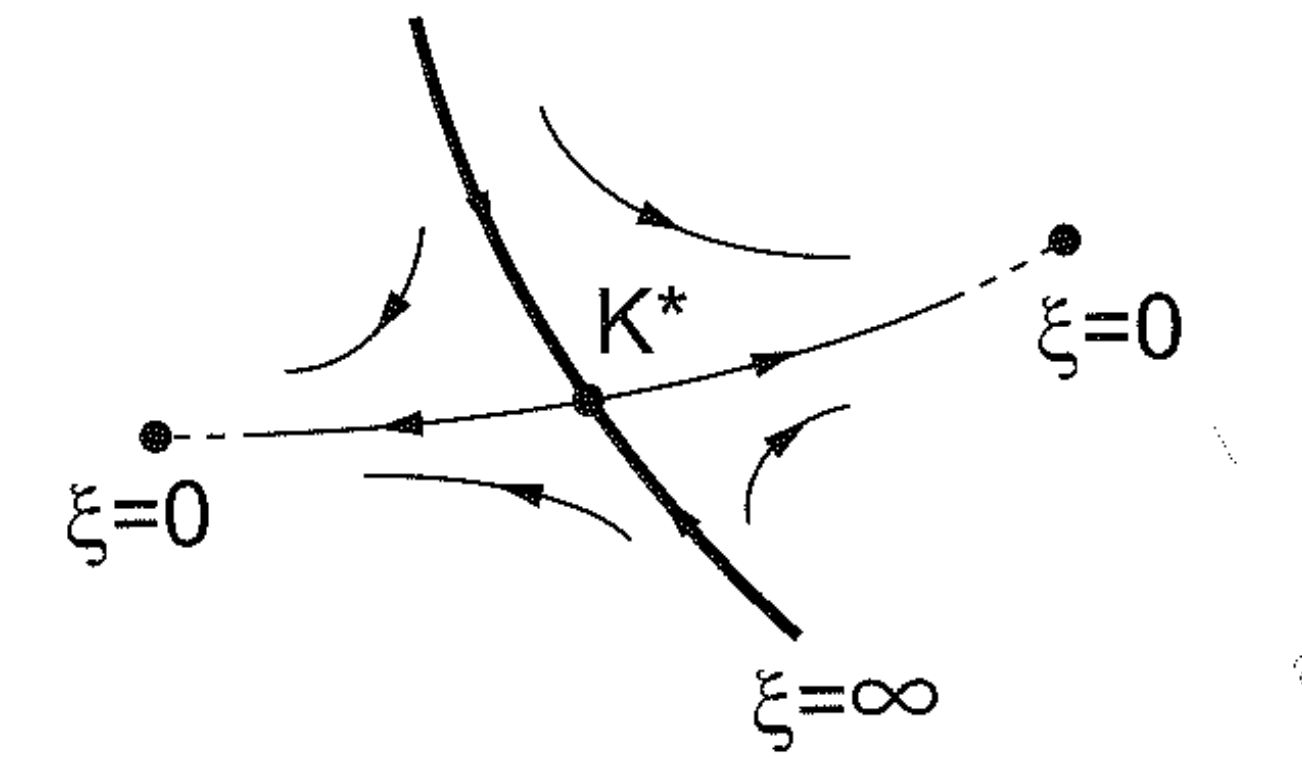
\includegraphics[width=100mm]{kk.png}
    \end{center}
    \caption{相図}
    \label{fig:kk}
\end{figure}

\subsubsection{スケーリングと普遍性}
固定点の近くでのくりこみ群変換を見ることで、臨界現象の性質を調べる。いま、固定点を$K^*$とし、その近傍の点を$K = K^* + \delta K$とする。このとき、結合定数の変化は、
\begin{align}
    K' = K^* + \delta K' 
\end{align}
と変化する。$K$が$K^*$に十分近いとき、$\delta K'$は$\delta K$に比例すると考えられる。すなわち、
\begin{align}
    \delta K' _{\alpha} = \sum_{\beta}(\hat{T}^{(b)})_{\alpha \beta} \delta K_{\beta}
\end{align}
と書ける。この変換の性質を見るために、行列$\hat{T}^{(b)}$を対角化することを考える。いま、右固有ベクトル及び左固有ベクトルをそれぞれ$R_{\mu}, L_{\mu}^{\top}$とすると、固有値$\lambda_{\mu}^{(b)}$をもちいて、
\begin{align}
    L_{\mu}^{\top} \hat{T}^{(b)} &= L_{\mu}^{\top} \lambda_{\mu}^{(b)}\\
    \hat{T}^{(b)} R_{\mu} &= \lambda_{\mu}^{(b)} R_{\mu}
\end{align}
と書くことができる。これらの固有ベクトルを用いて、
\begin{align}
    \hat{L}^{\top} = 
    \begin{pmatrix}
        L_1^{\top} \\
        L_2^{\top} \\
        \vdots
    \end{pmatrix}
    \quad 
    \hat{R} =
    \begin{pmatrix}
        R_1 & R_2 & \cdots
    \end{pmatrix}
\end{align}
とすると、右固有ベクトルについての固有値問題より、
\begin{align}
    \hat{L}^{\top} \hat{T}^{(b)} \hat{R} =
    \begin{pmatrix}
        L_1^{\top}\\
        L_2^{\top}\\
        \vdots
    \end{pmatrix}
    \begin{pmatrix}
        \lambda_1^{(b)} R_1 & \lambda_2^{(b)} R_2 & \cdots
    \end{pmatrix}
\end{align}
となる。また、左固有ベクトルについての固有値問題より、
\begin{align}
    \hat{L}^{\top} \hat{T}^{(b)} \hat{R} =
    \begin{pmatrix}
        \lambda_1^{(b)} L_1^{\top}\\
        \lambda_2^{(b)} L_2^{\top}\\
        \vdots
    \end{pmatrix}
    \begin{pmatrix}
        R_1 & R_2 & \cdots
    \end{pmatrix}
\end{align}
となる。このとき、異なる固有値の固有ベクトルは直交する。また、規格化$L^{\top}_\mu R_{\mu}=1$をとるにより、
\begin{align}
    \hat{L}^{\top} \hat{R} = I
\end{align}
となることがわかる。%TODOこれの前に少しだけ書き足す。
したがって、
\begin{align}
    \hat{T}^{(b)} = \hat{R} \hat{\Lambda}^{(b)} \hat{L}^{\top}
\end{align}
と書ける。ただし、$\hat{\Lambda}^{(b)}$は対角行列であり、その対角成分は$\lambda_{\mu}^{(b)}$である。このとき、
いま、
\begin{align}
    \delta K' = \hat{T}^{(b)} \delta K
\end{align}
であったから、これの左から$\hat{L}^{\top}$をかけると、
\begin{align}
    \hat{L}^{\top} \delta K' &= \hat{L}^{\top} \hat{T}^{(b)} \delta K\\
    &= \hat{\Lambda}^{(b)} \hat{R}\Lambda^{(b)} \hat{L}^{\top} \\
    &= \hat{\Lambda}^{(b)} \hat{L}^{\top} \delta K
\end{align}
となる。ここで、$\delta K, \delta K'$をそれぞれ右固有ベクトルの線形結合で表すと、
\begin{align}
    \delta K &= \sum_{\mu} g_{\mu} R_{\mu}\\
    \delta K' &= \sum_{\mu} g'_{\mu} R_{\mu}
\end{align}
と書ける。このとき、
\begin{align}
    \sum_{\mu} g'_{\mu} R_{\mu} &= \hat{\Lambda}^{(b)} \hat{L}^{\top} \qty(\sum_{\mu} g_{\mu} R_{\mu})\\
    &= \sum_{\mu} g_{\mu} \Lambda_{\mu}^{(b)} \\
    &= \sum_{\mu} \lambda_{\mu}^{(b)} g_{\mu} R_{\mu}
\end{align}
となる。したがって、
\begin{align}
    g'_{\mu} = \lambda_{\mu}^{(b)} g_{\mu}
\end{align}
となることがわかる。このとき、$g_{\mu}$をスケーリング変数と呼ぶ。

無限小のくりこみ群変換を考えてみる。今、くりこみ群変換の結合律から、
\begin{align}
    \hat{T}^{(b_2)} \hat{T}^{(b_1)} = \hat{T}^{(b_1b_2)}
\end{align}
となる。ここで、$b_1 = b$, $b_2 = 1 + \epsilon$とし、変換の生成子$\hat{X}$を、
\begin{align}
    \hat{X} \hat{T}^{(b)} = 1 + \epsilon \hat{X} 
\end{align}
とすると、
\begin{align}
    (1 + \epsilon \hat{X}) \hat{T}^{(b)} &= \hat{T}^{(b+ b\epsilon)}\\
    \hat{X} \hat{T}^{(b)} &=  \frac{\hat{T}^{(b+ b\epsilon)} - \hat{T}^{(b)}}{\epsilon} \to b \pdv{\hat{T}^{(b)}}{b}
\end{align}
となる。したがって、
\begin{align}
    \hat{T}^{(b)} = b^{\hat{X}} 
\end{align}
と書ける。したがって、$\hat{T}^{(b)}$の固有値は、$\hat{X}$の固有値$x_{\mu}$をもちいて、
\begin{align}
    \lambda_{\mu}^{(b)} = b^{x_{\mu}}
\end{align}
と書ける。このとき、スケーリング変数は、
\begin{align}
    g'_{\mu} = b^{x_{\mu}} g_{\mu}
\end{align}
となる。
$x_{\mu}$は、固有値のスケーリング次元と呼ばれ、$x_{\mu} > 0$のとき、スケーリング変数$g_{\mu}$を\textbf{有意な変数}と呼ぶ。また、$x_{\mu} < 0$のときは\textbf{有意でない変数}と呼び、$x_{\mu} = 0$のときは\textbf{中立変数}と呼ぶ。\\
有意な変数は、くりこみ群変換を繰り返すことで大きくなっていき、固定点から離れていく。逆に、有意でない変数は小さくなっていき、固定点に近づく。固定点付近でのハミルトニアンは、
\begin{align}
    \mathcal{H} &= \sum_{\alpha} K_{\alpha} S_{\alpha}\\
    &= \sum_{\alpha} K_{\alpha}^* S_{\alpha} + \sum_{\alpha} \delta K_{\alpha} S_{\alpha}\\
    &= \sum_{\alpha} K_{\alpha}^* S_{\alpha} + \sum_{\mu} g_{\mu} \phi_{\mu} \label{eq:ham}
\end{align}
と書ける。ただし、
\begin{align}
    \phi_{\alpha} = \sum_{\alpha} (R_{\mu})_{\alpha} S_{\alpha}
\end{align}
であり、スケーリング演算子と呼ばれる。(\ref{eq:ham})の第二項は、$g_{\mu}$が有意かどうかによって振る舞いが変わり、有意な変数の場合はくりこみによって増加し、有意でない場合については減衰する。\\
また、固定点周りの自由エネルギーについて考える。
\begin{align}
    f(K^* + \delta K) := f(K^*;g)
\end{align}
とすると、前の話から、以下が成立する。
\begin{align}
    f(K^*;g_1, g_2, \cdots) = f(K^*;b^{x_1}g_1, b^{x_2}g_2, \cdots)
\end{align}
ここで、$g_1,g_2$が有意な変数であり、他は有意でない変数であるとすると、くりこみを繰り返すことでこの関数を二変数関数とみなすことができ、
\begin{align}
    f(K^*;g_1, g_2) = f(K^*;b^{x_1}g_1, b^{x_2}g_2)
\end{align}
となる。これは、前の章で出てきたスケーリングの話と一致する。このときの基本変数は、$K$ではなく、対角化することによって現れた$g$であることに注意されたい。
この時の相図は以下のようになる。
\begin{figure}[H]
    \begin{center}
    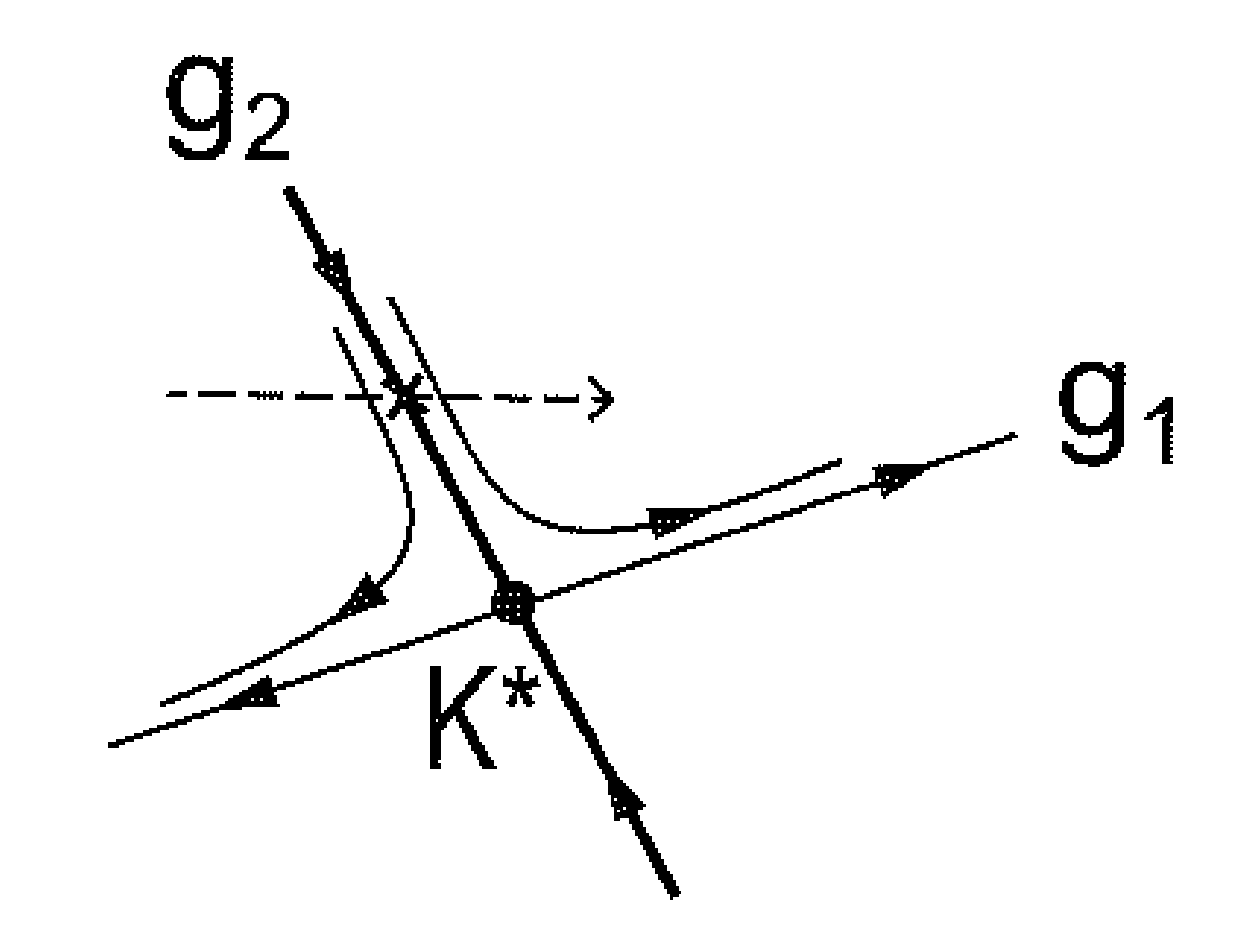
\includegraphics[width=100mm]{g.png}
    \end{center}
    \caption{相図}
    \label{fig:three}
\end{figure}
以上より、有意でない変数を無視することによって、くりこみ群変換の考え方からスケーリング理論を導くことができた。

\subsection{くりこみ群方程式}
$b$が離散値ではなく連続値をとる場合を考える。このとき、無限小のくりこみ群変換をを考えることで、微分方程式を導くことができる。\\
いま、結合定数$K$に依存する物理量$f$が、
\begin{align}
    f(K_1, K_2, \cdots) = Zf(K'_1, K'_2, \cdots)
\end{align}
を満たすとする。この両辺に$b\pdv{b} = \pdv{\ln b}$をかけ、$b=1$とすると、
\begin{align}
    \qty(b\pdv{Z}{b} + \sum_{\alpha} \beta_{\alpha} \pdv{K_{\alpha}} )f(K_1, K_2, \cdots) = 0 \label{eq:ku}
\end{align}
となる。\footnote{$b=1$で$Z=1$}ただし、
\begin{align}
    \beta_{\alpha} = b\pdv{K_{\alpha}}{b} = \pdv{K_{\alpha}}{\ln b} \label{eq:beta}
\end{align}
であり、$\beta$関数と呼ぶ。(\ref{eq:ku})はくりこみ群方程式と呼ばれ、関数$f$の変化を表す。また、(\ref{eq:beta})は、くりこみ群変換による結合定数の変化を表す。\\
\begin{figure}[H]
    \begin{center}
    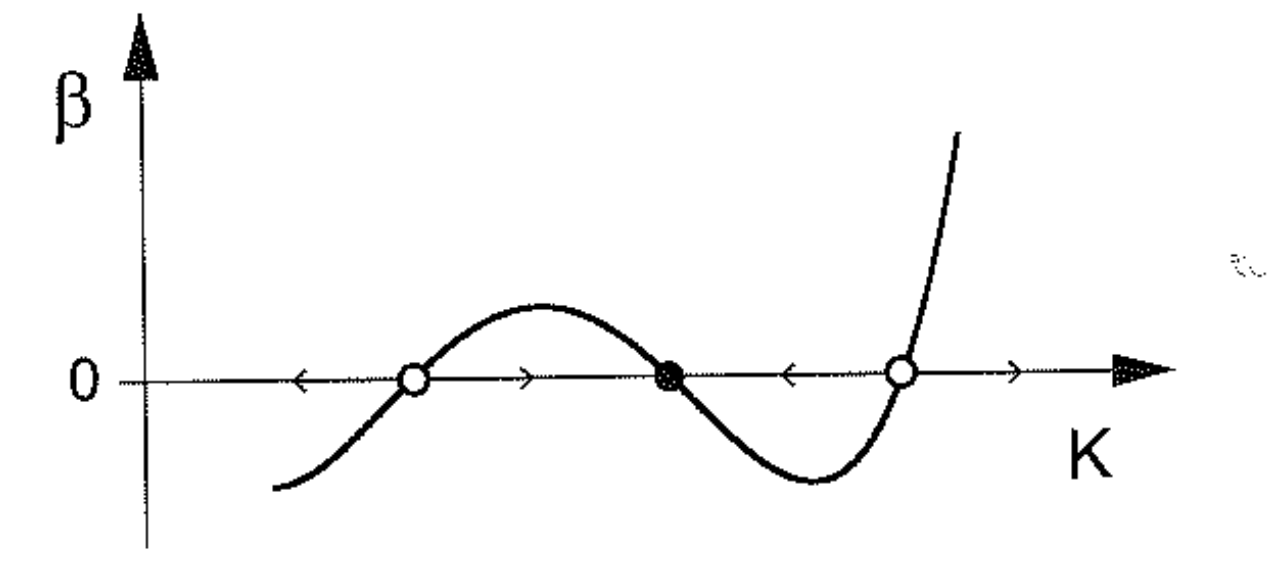
\includegraphics[width=100mm]{k.png}
    \end{center}
    \caption{くりこみ群方程式}
    \label{fig:four}
\end{figure}
$\beta>0$のとき、$K$はくりこみ群変換によって大きくなる。また、$\beta<0$のとき、$K$はくりこみ群変換によって小さくなる。したがって、図(\ref{fig:four})のように、
$\beta$が単調増加するところでは固定点から離れる方向に流れ、単調減少するところでは固定点に近づく方向に流れる。これは、前に見たくりこみ群の流れに対応する。\\

固定点の周りでの$K$の変換素行を考える。いま、
\begin{align}
    \delta K'_\alpha = \sum_{\beta} (\hat{T}^{(b)})_{\alpha \beta} \delta K_{\beta}
\end{align}
および、
\begin{align}
    \hat{T}^{(b)} = b^{\hat{X}}
\end{align}
であるから、
\begin{align}
    \beta_{\alpha} = \sum_{\alpha} \hat{X}_{\alpha \alpha'} K_{\alpha'}
\end{align}
となる。$\hat{X}$の対角化により、$\delta K = \sum_{\mu} g_{\mu} R_{\mu}$を用いると、
\begin{align}
    \beta_{\mu} = x_{\mu} g_{\mu}
\end{align}
となる。したがって、ベータ関数の固定点の近くでの傾きがスケーリング次元となることがわかる。とくに、$g_{\mu}$が有意な変数であれば$x_{\mu}$は正であり、くりこみ群変換により固定点から離れていく。また、$g_{\mu}$が有意でない変数であれば$x_{\mu}$は負であり、くりこみ群変換により固定点に近づいていく。\\
とくに、ベータ関数や$Z$が与えられたときは、具体的にスケーリング関数を計算することができる。
\end{document}